\section{Résultats} % (fold)
\label{sec:résultats}

\paragraph{Une amélioration nette du protocole.} % (fold)
\label{par:proto}
La première chose qui saute aux yeux dans les gels d'éléctrophorèse obtenus est la nette amélioration de l'amplification des fragments de grande taille, notamment pour les profils de type \textit{wMel} (Cf. Figure \ref{fig:wMelcomp}). 
\begin{figure}[tb]
	\begin{center}
		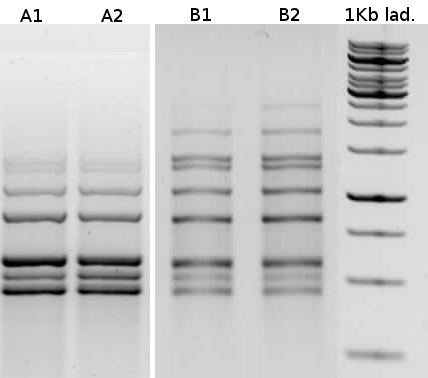
\includegraphics[width=80mm]{images/wMel_comp.png}
	\end{center}
	\caption{Comparaison des deux protocoles sur wMel (\esp{Wolbachia} de \esp{D. melanogaster})~:
	A1 et A2 : Ancien protocole\cite{memHH}~;
	B1 et B2 : Nouveau protocole, avec accuTaq}
	\label{fig:wMelcomp}
\end{figure}
% paragraph proto (end)

\paragraph{Polymorphisme} % (fold)
\label{par:polymorphisme}

% paragraph polymorphisme (end)

% section r_sultats (end)

\section{Conclusion \& Perspectives} % (fold)
\label{sec:ccl}
Afin de tirer des conclusions complètes sur les tranferts horizontaux, il faut encore attendre les résultats de transposon-display sur des lignées de \esp{L. heterotoma} infectées par une seule souche de \esp{Wolbachia}.
Nous ne possédons pas encore ces lignées, mais une seconde partie de ce stage, non développée ici; a consisté à démarrer un traitement antibiotique ménagé sur des \esp{L. heterotoma} tri-infectées (statut d'infection sauvage), afin d'obtenir des lignées présentant un statut d'infection différent 
% section conclusion_&_perspectives (end)
